\documentclass{beamer}
\usepackage[utf8]{inputenc}
\usepackage[]{polski}
\mode<beamer>{
\usetheme{Frankfurt}
\setbeamertemplate{navigation symbols}{}
}
\mode<handout>{
\usepackage{pgfpages}
\pgfpagesuselayout{4 on 1}[a4paper, border shrink=10mm, landscape]
\usetheme{default}
}

\title{Capacitated Vehicular Routing Problem}
\subtitle{Problem rozwożenia kontenerów}
\author{Aleksander Balicki, Łukasz Zapart}
\institute{Instytut Informatyki}
\date{\today}

\begin{document}
\mode*
\begin{frame}
\titlepage
\end{frame}

\begin{frame}
\tableofcontents[hideallsubsections]
\end{frame}


\section{Specyfikacja problemu}
\subsection{Oryginalna specyfikacja}
\begin{frame}
\frametitle{Oryginalna specyfikacja}
	Na placu znajduje sie pewna liczba kontenerów, które należy rozwieść samochodem do odbiorców. Samochód jednocześnie zabiera 3 kontenery. Zaplanować trasy samochodu, tak aby liczba przejechanych kilometrów była minimalna. (Jak rozwiązać ten problem, gdy mamy do dyspozycji kilka samochodów?)
\end{frame}

\subsection{Uściślenie specyfikacji}
\begin{frame}
\frametitle{Uściślenie specyfikacji}
	Na $n$-wierzchołkowym grafie z wagami na krawędziach i wyróżnionym wierzchołkiem $1$, musimy znaleść $k$ prawie rozłącznych cykli (wszystkie spotykają się w wierzchołku $1$), pokrywających cały graf.

	$n$ - liczba odbiorców
	$k$ - liczba ciężarówek

	Wymaga to założenia, że:
	\begin{itemize}
		\item żaden pakunek nie będzie podzielny,
		\item każdy pakunek ma objętość mniejszą niż dowolna ciężarówka.
	\end{itemize}
\end{frame}

\section{Model matematyczny}
\subsection{Dane wejściowe}
\begin{frame}
\frametitle{Dane wejściowe}
\begin{itemize}
    \item $d_i$ - liczba pakunków do zawiezienia do odbiorcy $i$, gdzie $i \in N = \{2, \dots, n\}$
    \item $k$ - liczba ciężarówek
    \item $C$ - pojemność jednej ciężarówki
    \item $c_{ij}$ - koszt dojazdu z miejsca $i$ do $j$, gdzie $i, j \in N \cup \{1\}$, a $1$ to wierzchołek startowy
\end{itemize}
\end{frame}

\subsection{Program całkowitoliczbowy}
\begin{frame}
\frametitle{Program całkowitoliczbowy}
\begin{itemize}
    \item[] $\displaystyle \min \sum_{e \in E} c_e x_e$
    \item[] $\displaystyle \sum_{e=\{1,j\} \in E} x_e = 2k$
    \item[] $\displaystyle \sum_{e=\{i,j\} \in E} x_e = 2 \;\;\; \forall i \in N$
    \item[] $\displaystyle \sum_{e=\{i,j\} \in E, i \in S, j \not\in S} x_e \geq 2\lceil (\sum_{i\in S} d_i)/C \rceil \;\;\; \forall S \subset N, |S| > 1$
    \item[] $\displaystyle 0 \leq x_e \leq 1 \;\;\; \forall e = \{i,j\} \in E, i,j \neq 1$
    \item[] $\displaystyle 0 \leq x_e \leq 2 \;\;\; \forall e = \{1,j\} \in E$
    \item[] $\displaystyle x_e \in Z \;\;\; \forall e \in E$
\end{itemize}
\end{frame}

\subsection{Otrzymany wynik}
\begin{frame}
\frametitle{Otrzymany wynik}
Otrzymany wynik składa się z:
\begin{itemize}
    \item $x_e \in \{0,1,2\}$ -- ile razy ciężarówka musi przejechać przez drogę $e$
    \item $Y = \min \sum_{e \in E} c_e x_e$ -- kosztu minimalnej drogi
    \item (opcjonalnie) obrazu grafu z zaznaczonymi drogami przejechanymi przez ciężarówki
\end{itemize}
\end{frame}

\section{Niewielki Przyklad}
\begin{frame}
\includegraphics[scale=0.4]{graphs/example.png}
\end{frame}

\section{Algorytm}
\subsection{Opis algorytmu}
\begin{frame}
\frametitle{Opis algorytmu}
The method solves the linear program without the integer constraint using the regular simplex algorithm. When an optimal solution is obtained, and this solution has a non-integer value for a variable that is supposed to be integer, a cutting plane algorithm is used to find further linear constraints which are satisfied by all feasible integer points but violated by the current fractional solution. If such an inequality is found, it is added to the linear program, such that resolving it will yield a different solution which is hopefully "less fractional". This process is repeated until either an integer solution is found (which is then known to be optimal) or until no more cutting planes are found.
At this point, the branch and bound part of the algorithm is started. The problem is split into two versions, one with the additional constraint that the variable is greater than or equal to the next integer greater than the intermediate result, and one where this variable is less than or equal to the next lesser integer. In this way new variables are introduced in the basis according to the number of basic variables that are non-integers in the intermediate solution but which are integers according to the original constraints. The new linear programs are then solved using the simplex method and the process repeats until a solution satisfying all the integer constraints is found. During the branch and bound process, further cutting planes can be separated, which may be either global cuts, i.e., valid for all feasible integer solutions, or local cuts, meaning that they are satisfied by all solutions fulfilling the side constraints from the currently considered branch and bound subtree.
\end{frame}

\section{Obliczenia testowe}
\begin{frame}
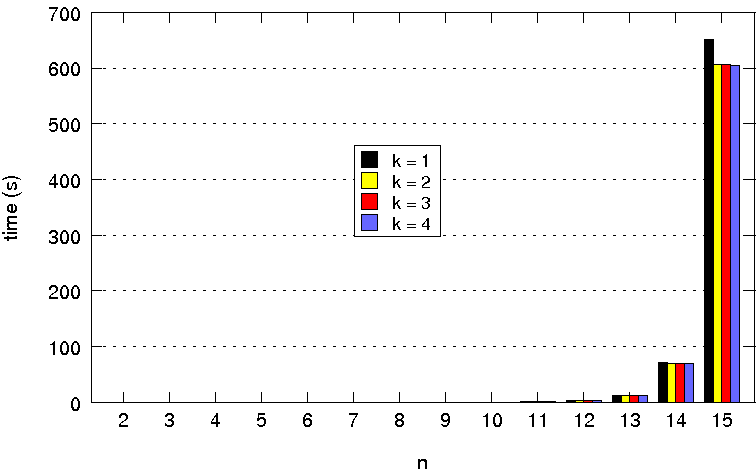
\includegraphics[scale=0.4]{times.png}
\end{frame}

\end{document}
